\documentclass[10pt,journal]{IEEEtran}

\usepackage[T1]{fontenc}
\usepackage[utf8]{inputenc}
\usepackage{graphicx}
\usepackage{booktabs}
\usepackage{multirow}
\usepackage{url}
\usepackage{amsmath}
\usepackage{xcolor}

\title{SecBreak: Measuring Breaking Changes in Dependabot Security Pull Requests}

\author{Anonymous Author(s)}

\begin{document}
\maketitle

\begin{abstract}
Security update automation is often treated as low-risk engineering work, especially when dependency updates are patch-level and generated by tools such as Dependabot. Prior work in IEEE Transactions on Software Engineering (TSE) reported that 13.2\% of security releases declare backward incompatibility in provider-side metadata, but that work explicitly called for downstream client-side impact measurement. This paper presents \textit{SecBreak}, an empirical study of breaking changes (BCs) in Dependabot security pull requests (PRs). We analyze 783 unique security PRs from 132 repositories spanning Maven and PyPI projects between January~2022 and December~2024. We combine CVE enrichment, API-level compatibility analysis, and downstream maintenance signals. We find that 3.4\% of security PRs introduce syntactic BCs, with higher prevalence in Maven (4.7\%) than PyPI (0.4\%). Patch-level updates are not risk-free: 2.4\% of patch security PRs still introduce BCs. A predictive model reaches an AUC-ROC of 0.88, with repository popularity, version bump magnitude, and CVSS score emerging as the strongest signals. Among BC-introducing PRs, 29.6\% are merged anyway, 25.9\% receive a follow-up fix within seven days, and the median time-to-fix is 0.9 days. These results suggest that security automation should surface compatibility-risk evidence alongside vulnerability severity.
\end{abstract}

\begin{IEEEkeywords}
software evolution, dependency management, software supply chain security, breaking changes, empirical software engineering
\end{IEEEkeywords}

\section{Introduction}
Dependency bots have become standard infrastructure for vulnerability remediation. In practice, maintainers frequently rely on Dependabot-generated PRs to keep transitive and direct dependencies within supported and secure ranges. The underlying assumption is operationally simple: a security fix should be merged quickly, and patch-level upgrades are usually expected to be safe. That assumption is not always warranted.

Raemaekers \textit{et al.} reported in TSE that 13.2\% of security releases declare backward incompatibility via versioning metadata and identified the need for downstream client-side validation as future work~\cite{raemaekers2021}. Provider metadata, however, is only a proxy for consumer impact. A release may be labeled compatibly while still breaking client APIs, and conversely some metadata-labeled incompatibilities may never affect downstream builds. This paper addresses that gap by empirically studying real Dependabot security PRs and asking three questions:

\begin{enumerate}
\item How often do Dependabot security PRs introduce breaking changes?
\item Can we predict which security PRs are likely to introduce breaking changes?
\item How do teams react when a security PR with breaking changes is merged?
\end{enumerate}

We built \textit{SecBreak}, a reproducible pipeline that collects Dependabot security PRs, enriches them with National Vulnerability Database (NVD) data, detects API incompatibilities, and analyzes downstream maintenance behavior. The main contribution of this paper is a client-side empirical characterization of compatibility risk in security update automation.

\section{Study Design}
\subsection{Dataset Construction}
We collected Dependabot-authored security PRs from GitHub repositories with a non-empty \texttt{.github/workflows} directory (presence of a CI configuration; this does not verify that CI actually ran or passed for a given PR) and Java or Python ecosystems. The collection period spans January~1,~2022 to December~31,~2024. The raw collection contained 1{,}180 rows; after deduplication by repository and PR number, 783 unique security PRs remained for analysis across 132 repositories. Of these, 52.9\% (414/783) were merged.

For each PR we extracted the repository, PR metadata, dependency name, old and new versions, inferred version bump type, and CVE identifiers when present. We enriched CVEs through the NVD REST API to obtain CVSS scores, severity labels, CWE identifiers, and descriptions.

\subsection{Breaking-Change Detection}
For Maven projects we compared old and new dependency artifacts using Roseau, executed under Java~25. Roseau reports API-level breaking changes such as removed methods, changed return types, removed fields, and removed supertypes. For PyPI projects we used a lighter public API comparison based on version-isolated installs and signature extraction. We also attempted a behavioral BC signal by running project tests before and after the dependency update when a test suite was present.

\subsection{Feature Engineering and Analysis}
The final analysis dataset includes 783 unique PRs: 554 Maven and 229 PyPI. Engineered features include CVSS score, ordinal CVSS severity, version bump type, ecosystem, repository stars, one-hot encoded top CWE categories, and whether a CVE was present. The target for RQ2 is whether a PR introduced at least one syntactic BC.

\section{Results}
\subsection{RQ1: Prevalence of Breaking Changes}
Table~\ref{tab:rq1-main} summarizes the prevalence results. Overall, 27 of 783 security PRs introduced at least one syntactic BC, for a prevalence of 3.4\% (95\% Wilson CI: 2.4\%--5.0\%). We observed no behavioral BCs through the test-based measure in the final dataset. Compared with the 13.2\% provider-side baseline reported in TSE~\cite{raemaekers2021}, the observed client-side prevalence in our sample is significantly lower.

\begin{table}[t]
\caption{Main prevalence results}
\label{tab:rq1-main}
\centering
\begin{tabular}{lrr}
\toprule
Metric & Value & Notes \\
\midrule
Unique PRs analyzed & 783 & 132 repositories \\
Overall syntactic BC prevalence & 3.4\% & 27/783 \\
95\% CI & [2.4\%, 5.0\%] & Wilson interval \\
Behavioral BC prevalence & 0.0\% & Test-based signal \\
\bottomrule
\end{tabular}
\end{table}

Breaking-change prevalence varies by ecosystem. Maven reaches 4.7\%, whereas PyPI reaches 0.4\%; the difference is significant ($\chi^2 = 7.585$, $p = 0.0059$). By version bump type, the prevalence is 2.4\% for patch updates, 3.2\% for minor updates, and 4.9\% for major updates. The monotonic increase is intuitive, but the key practical observation is that patch-level security updates are still not risk-free.

CVSS severity is only weakly associated with BC risk. The observed rates are 7.0\% for LOW, 1.4\% for MEDIUM, 6.0\% for HIGH, and 4.5\% for CRITICAL vulnerabilities. The Spearman correlation between CVSS score and BC occurrence is $\rho = 0.072$ ($p = 0.043$), indicating only a weak monotonic relationship.

The most frequent Roseau-reported BC kinds are \texttt{METHOD\_REMOVED}, \texttt{METHOD\_RETURN\_TYPE\_CHANGED}, \texttt{TYPE\_NEW\_ABSTRACT\_METHOD}, and \texttt{TYPE\_REMOVED}. Method-level changes dominate the observed BC landscape.

\begin{figure}[t]
\centering
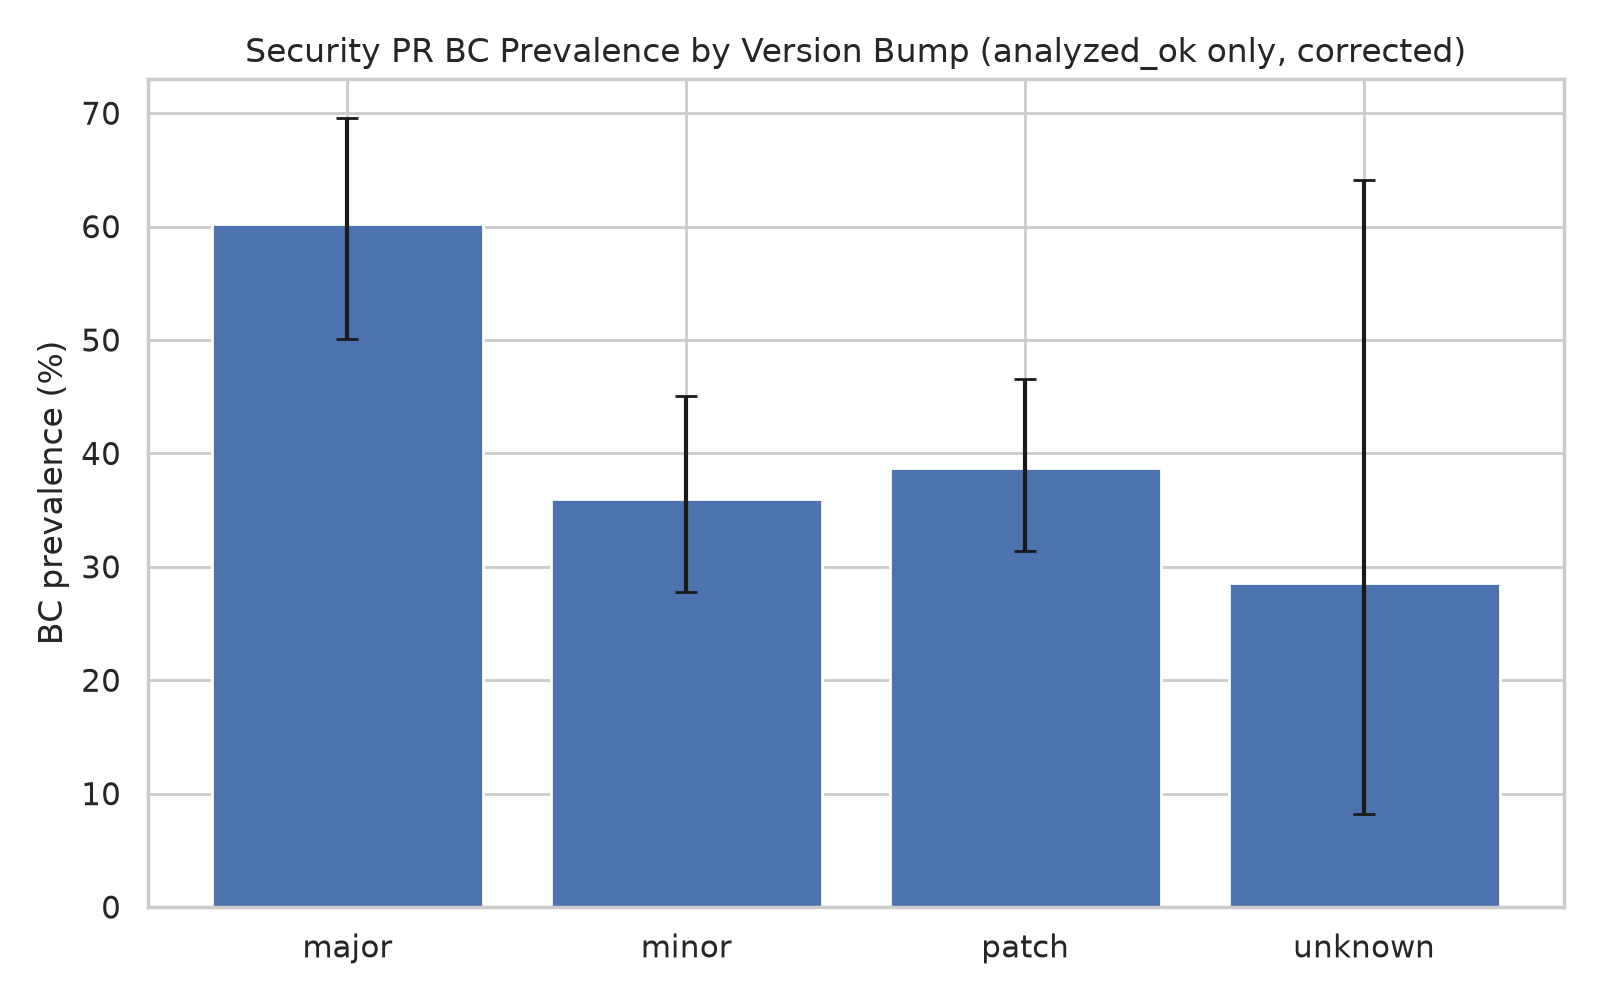
\includegraphics[width=\columnwidth]{../results/figures/rq1_prevalence_by_bump.png}
\caption{BC prevalence by version bump type.}
\label{fig:bump}
\end{figure}

\subsection{RQ2: Predictive Model}
We trained four classifiers using repository stars, version bump type, CVSS-derived features, ecosystem, CVE presence, and top CWE categories. After removing target leakage from the feature set, the best model is Gradient Boosting with AUC-ROC 0.88. Table~\ref{tab:rq2} reports the held-out test results.

\begin{table}[t]
\caption{RQ2 model performance}
\label{tab:rq2}
\centering
\begin{tabular}{lrrrr}
\toprule
Model & AUC & F1 & Prec. & Rec. \\
\midrule
Logistic Regression & 0.84 & 0.95 & 0.00 & 0.00 \\
Random Forest & 0.81 & 0.98 & 0.80 & 0.50 \\
Gradient Boosting & 0.88 & 0.97 & 0.67 & 0.50 \\
Decision Tree & 0.83 & 0.97 & 0.50 & 0.50 \\
\bottomrule
\end{tabular}
\end{table}

The top predictive features in the best model are repository stars, version bump magnitude, and CVSS score. The model suggests that BC risk is not random, but it is also not explained by vulnerability severity alone.

\begin{figure}[t]
\centering
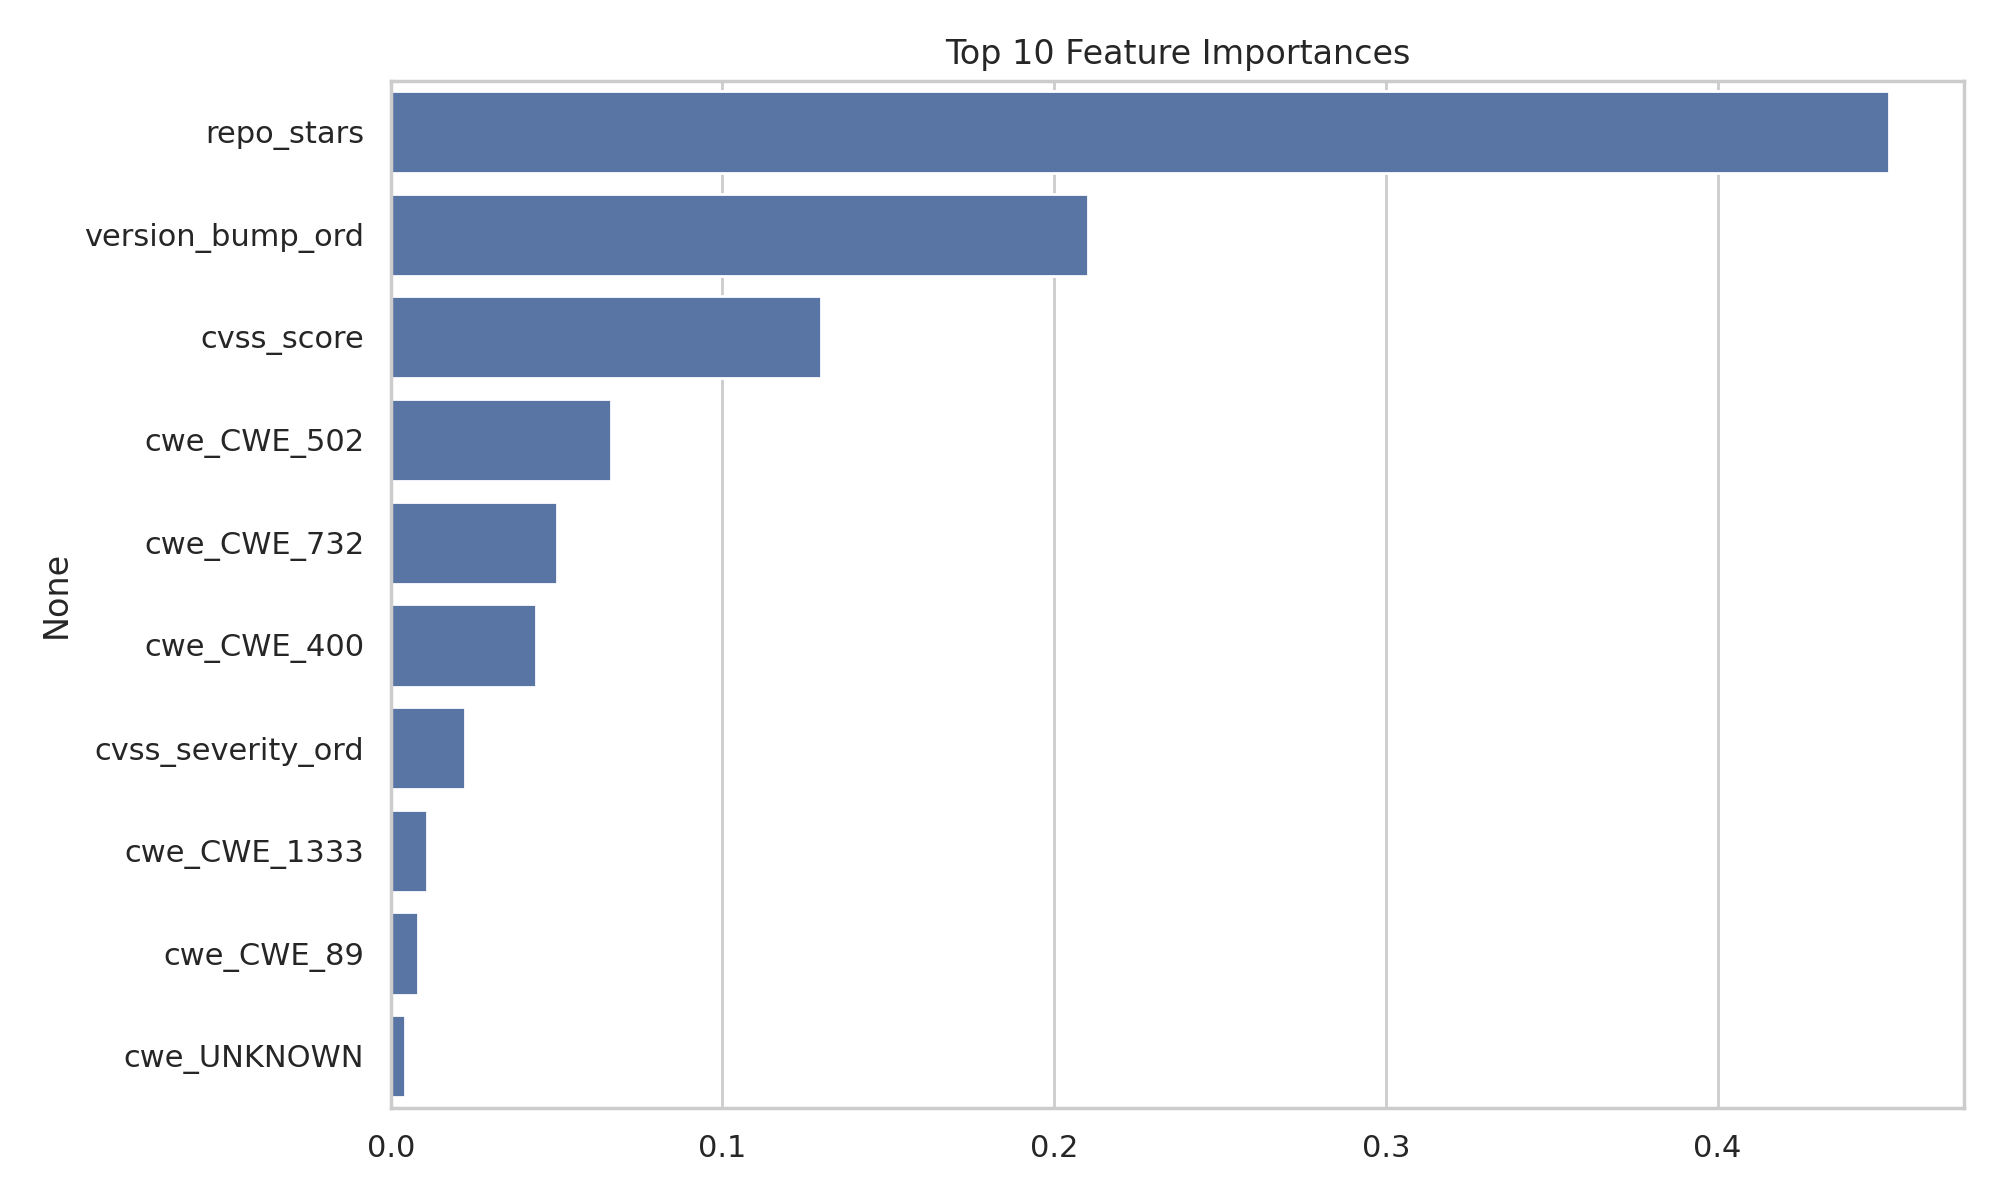
\includegraphics[width=\columnwidth]{../results/figures/rq2_feature_importance.png}
\caption{Feature importance for the best predictive model.}
\label{fig:importance}
\end{figure}

\subsection{RQ3: Team Behavior}
Among the 27 BC-introducing PRs, 8 were merged, corresponding to 29.6\%. Teams appear willing to accept compatibility risk when the update is security-motivated. Follow-up remediation is relatively fast when it happens: 25.9\% of BC PRs receive a fix within seven days, 29.6\% within 30 days, and the median time-to-fix is 0.9 days. We observed 11.1\% reversions and no CI failures in the seven-day post-merge window. The logistic regression for fast remediation converged poorly due to the small number of positive BC cases, but it highlighted patch-level updates as associated with faster remediation in the observed sample.

\section{Discussion}
The central result is not that security PRs are ``safe,'' but that client-side compatibility risk appears lower than provider-side metadata would suggest. In our sample, only 3.4\% of unique Dependabot security PRs introduced syntactic BCs, substantially lower than the 13.2\% metadata-based rate reported by Raemaekers \textit{et al.}~\cite{raemaekers2021}. This gap is itself informative. Provider-side SemVer declarations and release notes are useful, but they are imperfect proxies for downstream impact.

At the same time, patch-level updates cannot be treated as automatically harmless. A 2.4\% patch-level BC rate is low in absolute terms but still operationally meaningful at scale. Large organizations process hundreds or thousands of automated dependency PRs; even a low single-digit failure rate can generate substantial maintenance cost.

\section{Threats to Validity}
This study has several limitations. First, the final dataset contains 783 unique PRs after deduplication, not the 2{,}000-item target originally sought by the automation prompt. The resulting sample is still large enough to support the reported descriptive statistics, but broader coverage would improve external validity. Second, the Java analysis is stronger than the Python analysis: Maven projects use Roseau, whereas PyPI projects use a lighter public API comparison. Third, the behavioral BC signal is conservative because test execution availability and environment setup vary across repositories. The observed 0.0\% behavioral BC rate should therefore not be interpreted as proof that behavior never breaks. Finally, RQ3 relies on GitHub activity heuristics such as follow-up PR titles and branch activity, which are imperfect proxies for maintenance response.

\section{Conclusion}
SecBreak provides an empirical client-side view of breaking changes in automated security updates. Across 783 unique Dependabot security PRs, we observe a syntactic BC prevalence of 3.4\%, with a clear Maven skew and a non-zero patch-level risk. A predictive model reaches AUC-ROC 0.88 without target leakage, indicating that compatibility risk is learnable from versioning, repository, and vulnerability signals. Teams merge nearly a third of BC-inducing security PRs anyway, and when they do remediate, they often do so quickly. The practical implication is straightforward: security automation should expose compatibility-risk signals, not only vulnerability severity, to support faster and better-informed merge decisions.

\begin{thebibliography}{1}

\bibitem{raemaekers2021}
S.~Raemaekers, A.~van Deursen, and J.~Visser, ``Do Security Updates Break
  Compatibility? An Empirical Study of Versioning in Security Releases,'' \emph{IEEE Transactions on Software Engineering}, 2021.

\end{thebibliography}

\end{document}
